\documentclass[12pt]{article}

\usepackage{amsmath,amssymb}
\usepackage{graphicx}

\usepackage{setspace}
\onehalfspacing
\usepackage[margin=1in]{geometry}
\usepackage{hyperref}
\hypersetup{allcolors=blue, colorlinks=true}
\usepackage[utf8]{inputenc}
% Notation
% Mathematical functions
\newcommand{\isone}[1]{{\boldsymbol{1}\left( #1 \right)}}
\renewcommand{\Pr}[1]{{\mathbb{P}\left(#1\right) }}
\newcommand{\f}[1]{{f\left(#1\right) }}
\newcommand{\Prcond}[2]{{\mbox{Pr}\left(#1\vphantom{#2}\;\right|\left.\vphantom{#1}#2\right)}}
\newcommand{\fcond}[2]{{f\left(#1|#2\right) }}
\newcommand{\Expected}[1]{{\mathbb{E}\left\{#1\right\}}}
\newcommand{\ExpectedCond}[2]{{\mathbb{E}\left\{#1\vphantom{#2}\;\right|\left.\vphantom{#1}#2\right\}}}

\newcommand{\Likelihood}[2]{\text{L}\left(#1 \left|\vphantom{#1}#2\right.\right)}
\newcommand{\sufstats}[1]{s\left(#1\right)}
\renewcommand{\exp}[1]{\mbox{exp}\left\{#1\right\}}
\newcommand{\transpose}[1]{{#1}^\mathbf{t}}

% Objects
\newcommand{\params}{\theta}
\newcommand{\Params}{\Theta}
\newcommand{\Graph}{\mathbf{G}}
\newcommand{\graph}{\mathbf{g}}
\newcommand{\GRAPH}{\mathcal{G}}
\newcommand{\Adjmat}{Y}
\newcommand{\adjmat}{y}
\newcommand{\ADJMAT}{\mathcal{Y}}

\newcommand{\INDEPVAR}{\mathcal{X}}
\newcommand{\Indepvar}{X}
\newcommand{\indepvar}{x}

\newcommand{\normconst}{\kappa\left(\params, \Indepvar\right)}

% \graphicspath{{./fig/}}


%% NEED THIS FOR CANCY TEX
\usepackage{pstricks}

% Colors
\definecolor{USCCardinal}{HTML}{990000} % 153 0 0 in RGB
\definecolor{USCGold}{HTML}{FFCC00}
\definecolor{USCGray}{HTML}{CCCCCC}

% To use the function \sout
\usepackage{ulem}
\usepackage{tabularx, booktabs}

% \bibliography{bibliography.bib}

\title{Exponential Random Graph models for Little Networks\footnote{The authors would like to thank Garry Robins, Carter Butts, Johan Koskinen, Noshir Contractor, and Andrew Salughter for their valuable contributions to this work. The usual disclaimer applies.}}
\author{George G. Vega Yon\footnote{Corresponding author. email: \href{mailto:vegayon@usc.edu}{vegayon@usc.edu}} \and Kayla de la Haye}
\date{Department of Preventive Medicine\\University of Southern California\\ April 2019}

\begin{document}

\maketitle


\section{Introduction}

Statistical models for social networks have enabled researchers to study complex social phenomena that give rise to observed patterns of relationships among social actors, and to gain a rich understanding of the \textit{interdependent nature} of social ties and social actors \cite{Snijders2011,lusher2012exponential}. For example, this research has provided new insights into the role that attributes of social actors (e.g., their characteristics, beliefs, and decisions), and endogenous structural processes (e.g., social balance, and relationship reciprocity) play in shaping social networks in many different populations and social settings, and the influence that these social networks have, in turn, on individuals and groups. 

Much of this research has focused on social networks within medium to large social groups: from a couple of dozen students in a classroom, or colleagues in an organization; to larger social networks within schools, villages, and (online and offline) communities. To date, these advances in statistical models for social networks have rarely been applied to the study of small networks, despite small network data in teams, families, and personal (ego-centric) networks being common in many fields that study social phenomena. The study of small networks often uses descriptive statistics that summarize the structural features of the network; for example, the density, degree distribution, or triad count. However, researchers in these fields are often interested in testing hypotheses about \textit{why} small, localized social structures, such as reciprocity and balance, emerge in these small groups. A key limitation to this work has been the availability of statistical models for networks that can adequately test these hypotheses using an approach that is suited to the dependencies inherent in network data. In this paper, we propose an approach for applying one of the most widely used statistical models for social networks--exponential random graph models, or ERGM--to small graphs, to enable novel and rich research on ``little networks''. 



\def\fig1width{.45\linewidth}
\begin{figure}[tb]
\centering
\begin{tabular}{m{.2\linewidth}<\centering m{.4\linewidth}<\raggedright}
\toprule Representation & Description  \\ \midrule

\includegraphics[width=\fig1width]{terms/mutual.pdf} & Mutual Ties (Reciprocity)\linebreak[4]$\sum_{i\neq j}y_{ij}y_{ji}$  \\
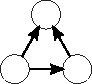
\includegraphics[width=\fig1width]{terms/ttriad.pdf} & Transitive Triad (Balance)\linebreak[4]$\sum_{i\neq j\neq k}y_{ij}y_{jk}y_{ik}$  \\

\includegraphics[width=\fig1width]{terms/homophily.pdf} & Homophily\linebreak[4]$\sum_{i\neq j}y_{ij}\mathbf{1}\left(x_i=x_j\right)$ \\
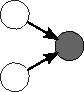
\includegraphics[width=\fig1width]{terms/nodeicov.pdf} & Covariate Effect for Incoming Ties\linebreak[4]$\sum_{i\neq j}y_{ij}x_j$ \\
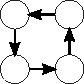
\includegraphics[width=\fig1width]{terms/fourcycle.pdf} & Four Cycle\linebreak[4]$\sum_{i\neq j \neq k \neq l}y_{ij}y_{jk}y_{kl}y_{li}$  \\
\bottomrule
\end{tabular}
\caption{\label{fig:ergm-structs}Besides of the common edge count statistic (number of ties in a graph), ERGMs allow measuring other more complex structures that can be captured as sufficient statistics. }
\end{figure}

\section{Exponential-Family Random Graph Models}

Exponential-Family Random Graph Models (ERGMs) are one of the most popular tools used by social scientists to understand social networks  \cite[and others]{Robins2007,Holland1981,Wasserman1996,Snijders2006}. In this family of models, an observed graph $\adjmat$, or more commonly put, its adjacency matrix representation, is characterized by a set of sufficient statistics, which we denote $\sufstats{}$, as follows:

\begin{equation}
\label{eq:ergm}
  \Prcond{\Adjmat = \adjmat}{\params, \Indepvar} = \frac{%
  	\exp{\transpose{\params}\sufstats{\adjmat, \Indepvar}}%	
  }{
  	\kappa\left(\params, \Indepvar\right)
  },\quad\forall \adjmat\in\ADJMAT
\end{equation}

\noindent Where $\normconst{} = \sum_{\adjmat\in\ADJMAT}\exp{\transpose{\theta}\sufstats{\adjmat, \Indepvar}}$ is the normalizing constant, and $\ADJMAT$ is the support of the model which is usually assumed to include all directed graphs of the same size as $\adjmat$, that are directed, and do not include self-ties. In this case, the size of $\ADJMAT$ equals $2^{n(n-1)}$ possible graphs. This makes the exact calculation of $\normconst{}$, and therfore of \eqref{eq:ergm}, extremely complicated to calculate. \autoref{fig:ergm-structs} shows some examples on structures (statistics) that can be used with ERGMs.

Modeling ``small networks'' is a topic mentioned several times in the literature on social network models  \cite{Wasserman1996,Frank1986,Snijders2011},  although much less frequently than studies of large networks, and applications of network models such as ERGMs to small networks is rare.\footnote{Perhaps because that, as put by \cite{Snijders2011}, small networks are considered to be ``uninteresting special cases''} Thus, ERGM methods have been developed to accommodate larger networks (although they do not scale well to ``very large'' networks of several thousand nodes or more). For example, rather than calculating the likelihood function using exhaustive enumeration (which we will refer as exact likelihood), the most popular software packages used for estimating these models apply simulation-based estimation methods.

As a consequence, the methods used to estimate ERGMs for large networks do not translate well to small network data (i.e., 10 or fewer nodes). The inference degeneracy problem \cite{Handcock2003} often encountered with these methods, even with large networks, is even more prevalent in the case of small networks. For example, if we are trying to estimate an ERGM in a network with only three nodes, in the scenario where the graph is directed and does not allow for self-ties, the chances of obtaining a graph with 1 or zero ties (emtpy or almost completely empty), or one with 5 or 6 ties (fully or almost fully connected) is about 20\% using a uniform sampler. The degeneracy problem is so common with small networks (e.g., 3 to 10 nodes) that practitioners typically cannot estimate ERGMs for small graphs. One work-around that is sometime attempted when multiple small networks are observed, is to aggregate the small networks into one large graph to obtain something similar to pooled estimates. Specifically, practitioners stack multiple adjacency matrices as a single matrix  building a block-diagonal data set, explicitly modeling the networks as independent by fixing the ``off diagonal'' components to 'impossible' (structural zeros). The problem with this approach is that the very set of constraints that are subscribed to the model make the sampling procedure complicated. 

To overcome this issue, we leverage the fact that in the case of small networks the likelihood function is tractable, and thus, we can directly estimate model parameters without using Markov Chain Monte Carlo (MCMC) methods, avoiding the convergence issues associated with inference degeneracy \cite{Handcock2003}. In this paper, we revisit ERGMs for small networks, which we define as those networks in which enumerating the entire support of the distribution is possible using modern computers (i.e., networks of size 3 to 6 nodes). We propose an estimation process that can be used in this type of application, and present results from an extensive simulation study evaluating the feasibility and validity of this method.

\section{\ergmitos{}: ERGMs for small networks}

In modern computers, calculating the exact likelihood function of an exponential random graph model for a small network becomes computationally feasible. This has an important implication: the estimation process of the parameters of an ERGMs of a small networks can be done directly without having to use simulations like modern methods do when fitting this kind of models. This way, besides of obtaining a better solution (in general), if the MLEs exists, we avoid the degeneracy problem. It is important to notice that, while the degeneracy problem is not completely avoided, we are indeed reaching a better situation compared to what we would get if we were using MC-MLE estimation, for example. One result by \cite[p. 7]{Handcock2003}, "[i]f the model used to simulate the graphs is not close enough to produce realizations that cover the observed values of the statistics, the MC-MLE will not exist even in cases where the MLE does.", in other words, while the non-existence of MLE estimates implies the non-existence of MC-MLE estimates, the opposite is not true.

Since most of small network data comes in the form of multiple networks--for example, families, small teams, ego-networks, etc.--assuming that the data generating process is shared across the sampled networks, then obtaining pooled estimates is a natural way of estimating of modeling the graphs. Pairing up the previous assumption with an independence independence across graphs, allows us calculating the exact likelihood function for pooled estimates by maximizing the following:

\begin{equation}
    \label{eq:ergm-pooled}
    \Prcond{\Adjmat_1 = \adjmat_1, \dots, \Adjmat_P = \adjmat_P}{\params, \Indepvar_1, \dots, \Indepvar_p} = \prod_{p=1}^P\frac{%
    		\exp{\transpose{\params}\sufstats{\adjmat_p, \Indepvar_p}}%	
    	}{
    		\kappa_p\left(\params, \Indepvar_p\right)
    	}
\end{equation}

\noindent Where $P$ denotes the number of networks used in the model. We call this model ERGMito\footnote{The \textit{ito}/\textit{ita} suffix is used in Spanish to denote small, or affection. We are particularly grateful to George Barnett who proposed the name during the North American Social Networks Conference on 2018.}.

One potential problem that we are not addressing with the pooled estimates is the problem of scalability, in particular, the interpretation of the constant parameter in the model, the edge count parameter. In the baseline case of estimating a density parameters using a single network, as pointed out in \cite{Krivitsky2011}, extrapolating or comparing those estimates in the context of a network with a different size may be a bit complicated in the sense that, if left as is, a fixed density parameter assumes a constant change in the average degree of the network, which may not be realistic in some scenarios, as instead it may be more natural to think that the degree holds constant. Still, the cases pointed out by \cite{Krivitsky2011} discuss situations in which the sizes of the networks range from a few dozens to a couple of thousands, which will not be the case here.

The simulations and model fitting were conducted using the R package \texttt{ergmito} which has been developed to implement the methods described in this work.

\section{Illustration with simulated data: fivenets}

\subsection{Data-generating-process and model fitting}

In what follows we will work with a toy data set generated using the data-generating-process of \ergmitos{}. This particular dataset, which we call ``fivenets'', is included in the in the R package \texttt{ergmito}\footnote{The R package is available to be downloaded at  \url{https://github.com/muriteams/ergmito}}. The dataset contains five simulated networks, each using the following model:

\begin{multline*}
\Prcond{\Adjmat = \adjmat}{\Indepvar_{\mbox{gender}}, \params} = \\
\frac{ %
    \exp{\params_{edges}\left(\sum_{i,j} \adjmat_{ij}\right) + %
    \params_{homophily}\left(\sum_{i,j} \adjmat_{ij}\isone{\Indepvar_{gender, i} = \Indepvar_{gender, j}}}\right) %
    }{%
    \normconst{}
    }
\end{multline*}

\noindent where $\params_{edges} = -2.0$ and $\params_{homophily} = 2$. Using the previous equation, we draw five networks of size five. In the case of the ``homophily'', parameter which is operationalized as the number of ties in which ego and alter have the same gender, before drawing the networks, we randomly generated the gender parameter to each vertex as a Bernoulli with parameter 0.5. \autoref{fig:fivenets} shows the five networks.

\begin{figure}[tb]
    \centering
    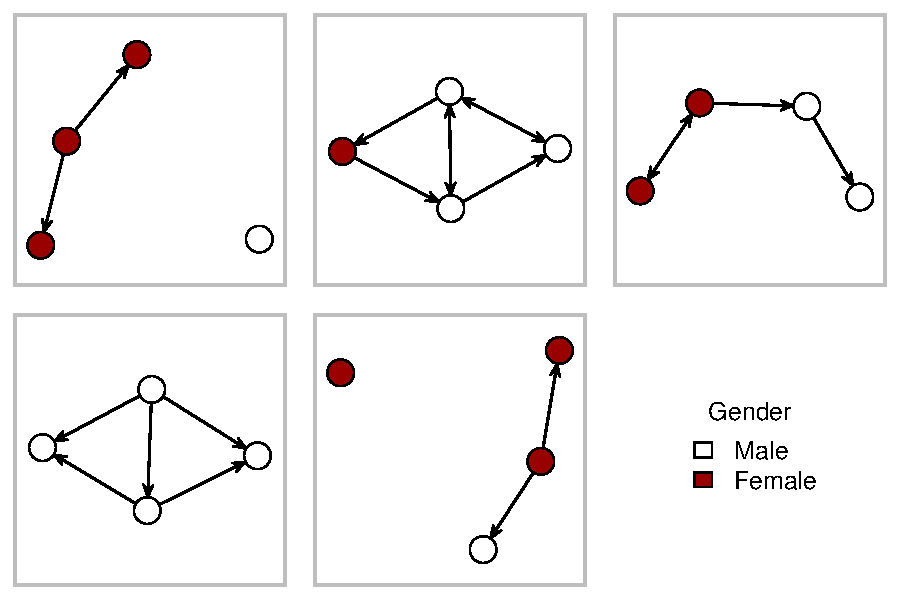
\includegraphics[width=.6\linewidth]{figures/fivenets_graphs.pdf}
    \caption{\label{fig:fivenets}Fivenets dataset. These graphs were randomly drawn from an ERGM distribution with parameters edgecount and homophily on gender equal to -2.0 and 2.0 respectively.}
    \label{fig:my_label}
\end{figure}


\autoref{table:coefficients} shows the estimation results of three different specifications of the model: (1) Homophily only, (2) Edgecount ($edges$) only, and (3) Full model (both parameters). As expected, model (3) as the best overall fit to the data. The 


\begin{table}
\begin{center}
\begin{tabular}{l c c c }
\hline
 & Homopholy & Edgecount & Full model \\
\hline
Edgecount             &          & $-0.69^{*}$ & $-1.70^{**}$ \\
                      &          & $(0.27)$    & $(0.54)$     \\
Homophily (on Gender) & $-0.12$  &             & $1.59^{*}$   \\
                      & $(0.34)$ &             & $(0.64)$     \\
\hline
AIC                   & 85.06    & 78.38       & 73.34        \\
BIC                   & 87.15    & 80.48       & 77.53        \\
Log Likelihood        & -41.53   & -38.19      & -34.67       \\
Num. networks         & 5        & 5           & 5            \\
\hline
\multicolumn{4}{l}{\scriptsize{$^{***}p<0.001$, $^{**}p<0.01$, $^*p<0.05$}}
\end{tabular}
\caption{Fitted ERGMitos using the fivenets dataset. As expected, the Full model (last column of the table) has overall a better fit of the data. More over, the 95\% level CI of each covers the true parameters: $\hat\theta_{edges} \in [-2.77, -0.64]$; $\hat\theta_{Homophily} \in [0.33, 2.85]$.}
\label{table:coefficients}
\end{center}
\end{table}


\subsection{Goodness-of-fit in \ergmitos}

Practitioners of ERGMs should be familiar with the goodness-of-fit diagnostic performed every time one of these models is fitted. In general, the most scrutinized statistic--and yet harder to obtain a good fit--is the distribution of shortest-path lengths. In the case of ERGMitos such statistic loses some relevance since, in general, the shortest-path lengths between any two nodes lies usually (or at least there is a high chance of) between 1 and 2 steps. Instead, we look directly at the fitted parameters in the model as the bare-minimum as showed in \autoref{fig:fivenets-gof}. An important difference from what is commonly done is that, instead of looking at a boxplot, since we are actually able to enumerate the full support of the model, we present a 90\% confidence interval per-statistic per network, comparing the fitted model's distribution with the observed parameters. A thorough discussion about this part of the ERGMitos is presented at the end of this paper.

An important advantage of the ERGMitos over ``regular'' ERGMs is that we can observe the surface of the log-likelihood over different combination of parameters in a rather straightforward way. This, together with the goodness-of-fit analysis should be a routine thing to be done after every ERGMito fit. \autoref{fig:fivenets-loglike} shows the surface of the log-likelihood function around the solution.

\begin{figure}[tb]
    \centering
    \caption{Goodness-of-fit in ERGMitos. In this case we are showing how do the observed sufficient statistics of each one of the 5 networks (x-axis) locate in the overall estimated distribution based on the fitted ERGMito. The gray lines in each box show the minimum and maximum value that the sufficient statistics can take in each one of the 5 networks, whereas the dotted lines provide a 90\% confidence interval. The dots are the observed statistics in each network.}
    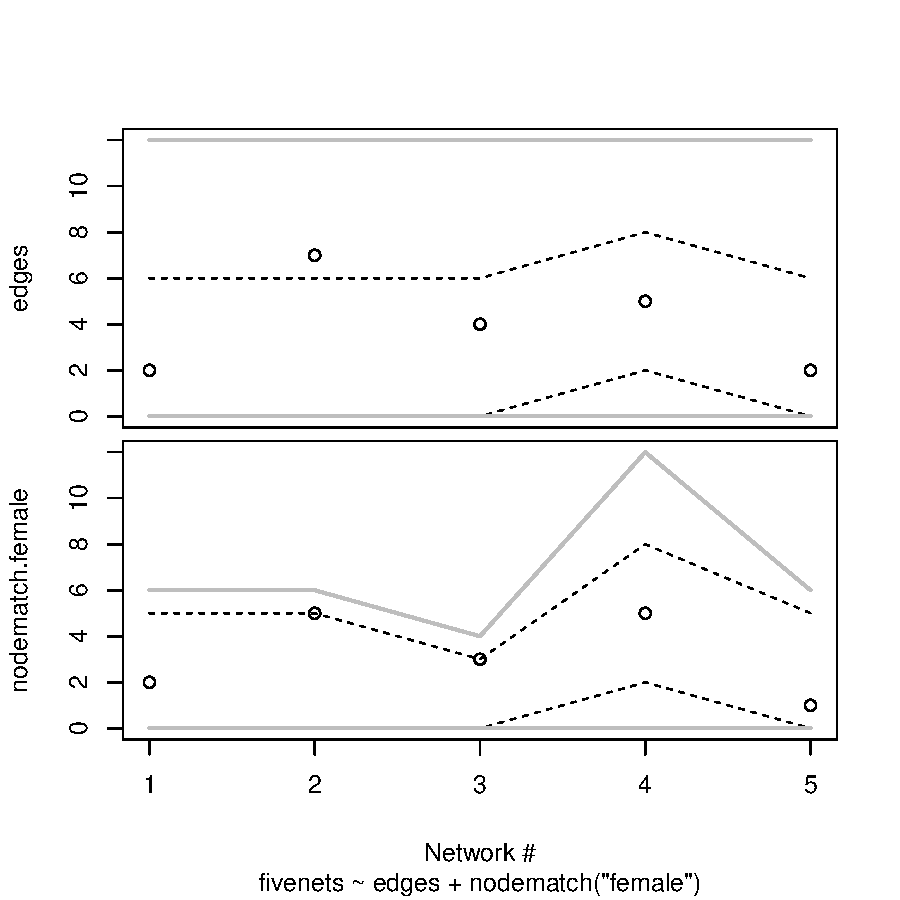
\includegraphics[width=.7\linewidth]{figures/fivenets_gof.pdf}
    \label{fig:fivenets-gof}
\end{figure}

\begin{figure}[tb]
    \centering
    \caption{Surface of the log-likelihood function of the pooled ERGMito model. Lighter colors represent higher values while darker ones represent lower values. The red dot corresponds to the location of the MLE estimate of the model.}
    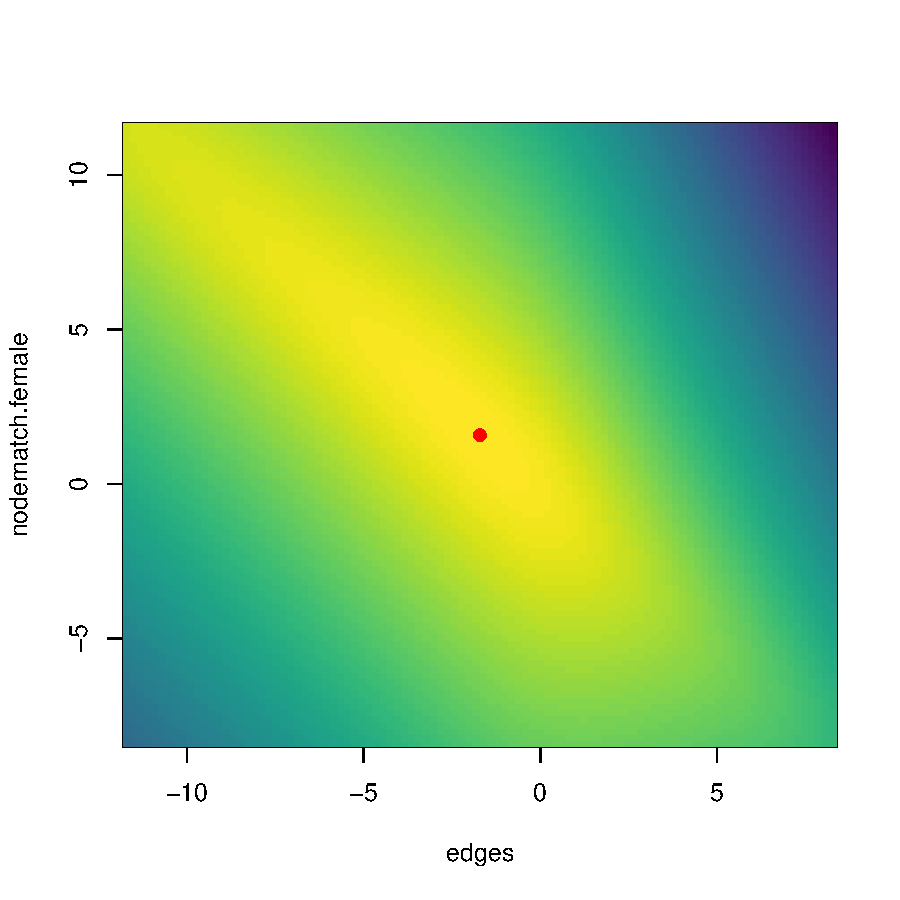
\includegraphics[width=.7\linewidth]{figures/fivenets_loglike.pdf}
    \label{fig:fivenets-loglike}
\end{figure}

\pagebreak
\section{Simulation study}

\subsection{Sampling groups of small networks}

We conducted a simulation study to explore the properties of MLE for small networks. Using the \texttt{ergmito} R package, we generated 100,000 samples of groups of small networks, each one with an average of 30 networks, which accounts to approximately 3 million small networks drawn from an ERGM distributions. In particular, to generate each one of the 100,000 samples we did the following:

\begin{enumerate}

\item Draw two numbers from a piece-wise Uniform with values in $[-4, -.1]\cup[.1, 4]$. These two correspond to the parameters \textbf{edgecount} ($\params_{edges}$) and number of \textbf{mutual ties} ($\params_{mutuality}$) for the sufficient statistics.

\item The number of networks included in the sample was obtained from 3 Poisson distributions with the parameter mean equal to 10, in particular, each one of those specified how many networks of sizes 3 ($n_3$), 4 ($n_4$), and 5 ($n_5$) would be generated. This implies that on average each sample has ten networks of each size, this is, a total of 30 networks per sample.

\item Finally we draw $n_3$, $n_4$, and $n_5$ networks of sizes 3, 4, and 5 respectively from ERGM distributions with parameters $(\params_{edges}, \params_{mutuality})$ (so all 3 network sizes share the same set of population parameters). Again, we repeated 1 through 3 100,000 times.
\end{enumerate}

Unfortunately, given the small size of these networks, it is easy to simulate population parameters that fell within the almost-degenerate (and actually, degenerate) region of the parameter space. Because of this reason, the final analysis only considers 54,995 samples. The next section discusses the results.

\subsection{Results}

\autoref{fig:bias} shows the empirical bias.

\autoref{fig:power} shows the empirical power level achieve for the estimator.

\begin{figure}
	\centering
	\caption{\label{fig:power}Empirical power by sample size and model parameter.}
	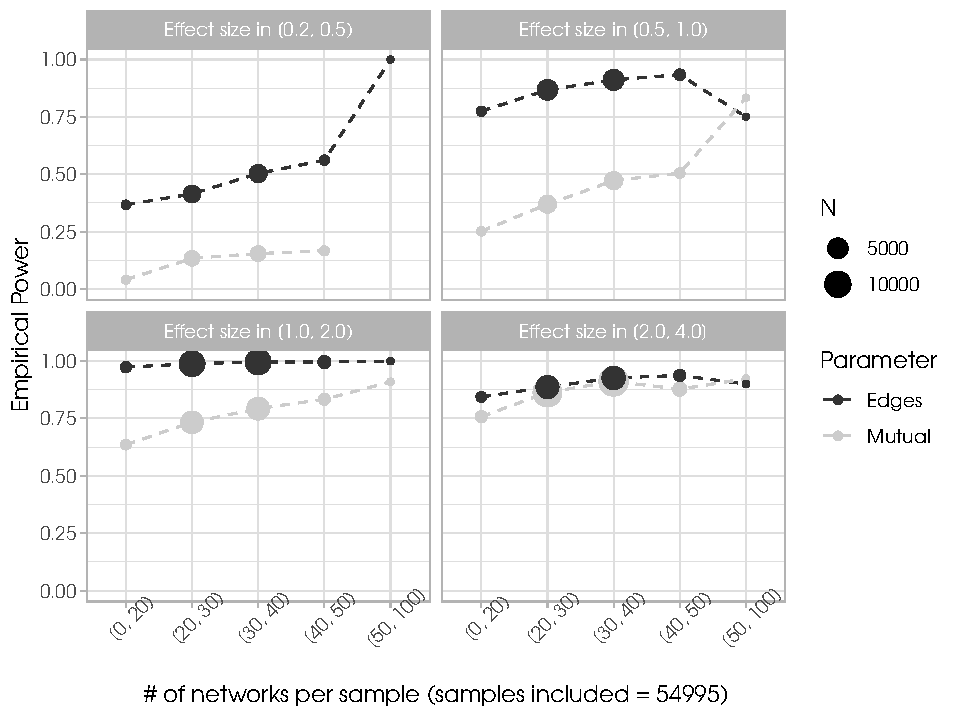
\includegraphics[width=.9\linewidth]{power-02-various-sizes-3-5.pdf}
\end{figure}

\begin{figure}
    \centering
    \caption{\label{fig:bias}Violin plots showing the empirical distribution of the bias per model parameter. In general we see that the parameter estimates' bias is centered around zero and in all but a few cases within the range [-1, 1]. Just like the figure on empirical power, this figure contains 54,995 samples.}
    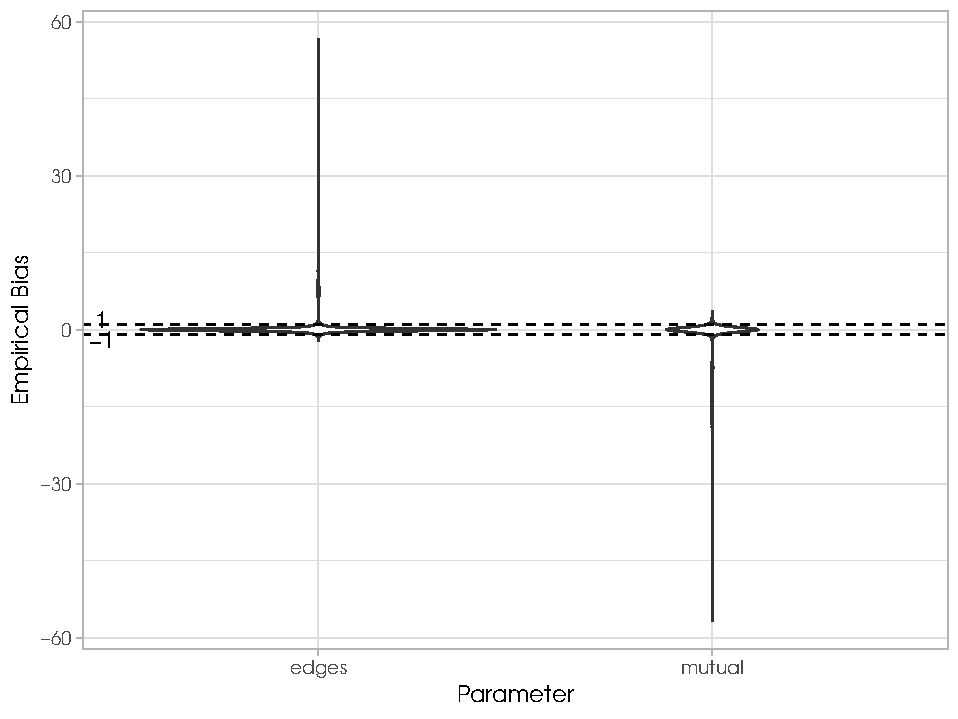
\includegraphics[width=.8\linewidth]{figures/bias-02-various-sizes-3-5.pdf}
\end{figure}

\pagebreak
\section{Discussion}

In this paper we have revisit the Exponential Family Random Graph Models for the case of small networks. Overall overlooked in estimation methods, ERGMs for small networks, or \ergmitos{} as we call them here, have the nice feature that, as a difference from other cases, can be estimated using Maximum Likelihood Estimation directly without having to recur to estimation via MCMC methods; this provides several benefits, mainly: (1) we avoid, if not completely, partially the model near-degeneracy problems that affect the aforementioned methods; (2) given the natural prevalence of samples of small networks like multiple families, small teams, or ego networks, pooling estimates come natural to the small networks setting, and indeed, we are able to estimate such models easily, all this improving accuracy and efficiency without losing anything.

There are still some unanswered questions regarding how to analyze \ergmitos{}. One of particular importance is how to evaluate goodness-of-fit. What are the statistics that we should look at, and what are the GOF statistics that are reasonable to expected in a model to consider it a ``good fit'' are questions that we need to keep thinking of. One point in favor is the fact that, as a difference from ``regular'' ERGMs, \ergmitos{} provide an rather simple way of conducting simulation studies, hence, for future work we should focus on answering these and other questions with it.

\section{Acknowledgements}

This material is based upon work support by, or in part by, the U.S. Army Research Laboratory and the U.S. Army Research Office under grant number W911NF-15-1-0577

Computation for the work described in this paper was supported by the University of Southern California’s Center for High-Performance Computing (hpcc.usc.edu).

\clearpage

\bibliographystyle{plain}
\nocite{vegayon2019,R,butts2016}
\bibliography{bibliography.bib}

\clearpage

\appendix

\section{MLE}

In order to improve accuracy of the estimation process, we use both the log-likelihood function and its gradient to find the MLEs. In particular, in this iteration of the manuscript we are using the BFGS quasi-newtonian optimization algorithm as provided by the R package stats in the optim function. In the general case, whether we have one or more networks (pooled estimates), the gradient of the log-likelihood function can be calculated as follows:

\begin{equation}
\sum_{p}\nabla l_p(\theta) = \transpose{\sufstats{\adjmat_p, \Indepvar_p}} - \frac{\transpose{Q_p}\left(\transpose{W_p} \circ \exp{Q_p \theta}\right)}{\kappa_p}
\end{equation}

Where $\sufstats{\adjmat, \Indepvar}$ is a vector of observed sufficient statistics (usually called target statistics), $Q$ is a matrix of sufficient statistics, in particular, the isomorphic sufficient statistics associated with the model, and $W$ is a vector of frequency weights.


\end{document}
